\documentclass[12pt]{article}
\usepackage[utf8]{inputenc}
\usepackage[margin=1.5cm]{geometry}
\usepackage{amsmath}
\usepackage{amssymb}
\usepackage{amsthm} % allows example and proof environment to be defined/used
\usepackage{cancel}
\usepackage{graphicx}
\usepackage{mathtools}
\usepackage{enumitem}  
\usepackage[normalem]{ulem}
\newtheorem*{esempio}{Esempio}
\DeclarePairedDelimiter{\abs}{\lvert}{\rvert}

\begin{document}

\section[Lezione 8 - Metodo di bisezione]{Lezione 8 - Introduzione alla soluzione numerica di equazioni non lineari, metodo di bisezione}
\subsection{Introduzione}
In questa e nelle prossime 3 lezioni ci occupiamo di un argomento classico del calcolo numerico, ovvero la soluzione numerica (cioè approssimata) di equazioni non lineari. Tratteremo 2 tipi di equazioni
\begin{itemize}
    \item $f(x)=0$, \uline{zeri} di funzione
    \item $x=\phi(x)$, equazioni di \uline{punto fisso}
\end{itemize}
che possiamo schematizzare coi seguenti disegni
\begin{center}
        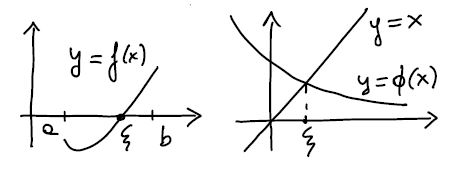
\includegraphics[width=0.5\textwidth]{1.JPG}\par
\end{center}
Il primo tipo corrisponde al calcolo di uno zero di una funzione (continua), cioè di un punto $\xi$ in cui $f$ si annulla. Il secondo tipo corrisponde invece al calcolo del punto fisso $\xi$ di una funzione (continua) $\phi$ e si può interpretare come calcolo dell'ascissa dell'intersezione del grafico della bisettrice del primo e terzo quadrante $y=x$ col grafico di $y=\phi(x)$.\\ In entrambi i casi daremo \uline{condizioni sufficienti} per \uline{l'esistenza} ($\exists$) e l'unicità (!) della soluzione in un dato intervallo e discuteremo, analizzando in dettaglio, tre metodi classici di soluzione: i metodi di \uline{BISEZIONE} e di \uline{NEWTON} (tangenti) per gli zeri e il metodo delle \uline{ITERAZIONI DI PUNTO FISSO}.
\newline
Cominciamo col ricordare alcuni risultati di esistenza e unicità nel caso della ricerca di zeri.

\subsubsection{TEOREMA (degli zeri di funzioni continue)}
\begin{center}
    \fbox{\begin{minipage}[t]{15cm}%
        Sia $f(x)\in C[a,b]$ (cioè $f$ continua nell'intervallo chiuso e limitato $[a,b]$ e $f(a)f(b)<0$ cioè $f$ cambia segno agli estremi)
        allora 
        \begin{center}
        $\exists \xi\in(a,b):f(\xi)=0$
        \end{center}
    \end{minipage}}
\end{center}
Osserviamo che tale zero può non essere unico:
\begin{center}
    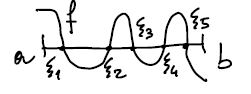
\includegraphics[width=0.3\textwidth]{2.JPG}\par
\end{center}
D'altra parte togliendo una delle ipotesi la condizione restante \uline{non} basta a garantire l'$\exists$
\begin{center}
    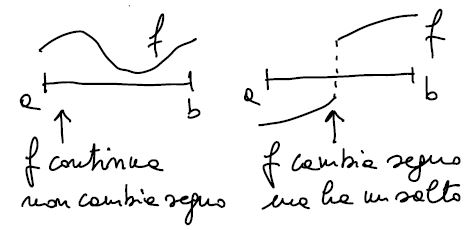
\includegraphics[width=0.5\textwidth]{3.JPG}\par
\end{center}
Ribadiamo che le condizioni \uline{non} sono \uline{necessarie}
\begin{center}
    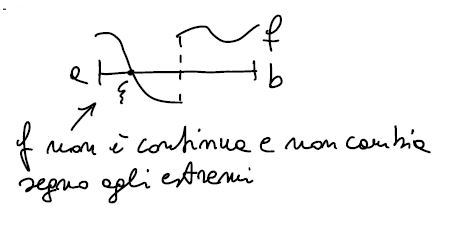
\includegraphics[width=0.5\textwidth]{4.JPG}\par
\end{center}
Diamo anche due classiche condizioni \uline{sufficienti} ciascuna delle quali garantisce l'\uline{unicità} dello zero
\begin{itemize}
    \item $f$ \uline{strettamente monotona} (strettamente crescente o decrescente in $[a,b]$
    \item $f \in C[a,b]$, $f(a)f(b)<0$ e $f$ \uline{strettamente convessa} o \uline{concava} in $[a,b]$
\end{itemize}
Nel caso in cui $f$ è derivabile in $[a,b]$ la monotonia stretta è legata al segno di $f'$

\[\begin{split}
    f'(x)>0  \text{ in }  [a,b] & \Rightarrow f \text{ strettamente crescente } \\
    f'(x)<0  \text{ in }  [a,b] & \Rightarrow f \text{ strettamente decrescente }
\end{split}\]
Ricordiamo che il viceversa è vero con la diseguaglianza non stretta,
\[\begin{split}
    f \text{ strettamente crescente } & \Rightarrow f'(x)\ge 0 \text{ in } [a,b] \\
    f \text{ strettamente decrescente } & \Rightarrow f'(x)\le 0 \text{ in } [a,b] 
\end{split}\]
come si vede ad esempio con la funzione $f(x)=x^3$ in $[-1,1]$
\begin{center}
    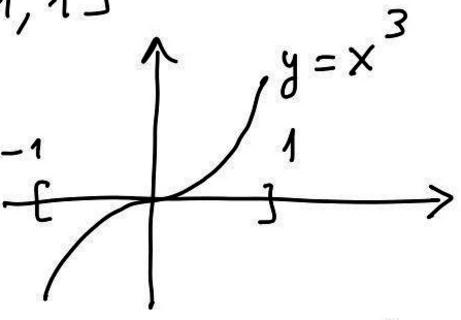
\includegraphics[width=0.3\textwidth]{5.jpg}\par
\end{center}
Per cui si ha che $f$ è strettamente crescente ma $f'(0)=3x^2|_{x=0}=0$.\\
Analogamente convessità e concavità stretta sono legate al segno di $f''$ quando $f$ è derivabile 2 volte in $[a,b]$
\[\begin{split}
    f''(x)>0  \text{ in }  [a,b] & \Rightarrow f \text{ strettamente convessa } \\
    f''(x)<0  \text{ in }  [a,b] & \Rightarrow f \text{ strettamente concava }
\end{split}\]
Di nuovo, il viceversa è vero con la disuguaglianza non stretta
\[\begin{split}
    f \text{ strettamente convessa } & \Rightarrow f''(x)\ge 0 \text{ in } [a,b] \\
    f \text{ strettamente concava } & \Rightarrow f''(x)\le 0 \text{ in } [a,b] 
\end{split}\]
($f(x) = x^4$ è  strettamente convessa in $[-1,1]$, $f''(0) = 0$)

Ribadiamo che le condizioni di unicità date sono solo sufficienti 
\begin{center}
    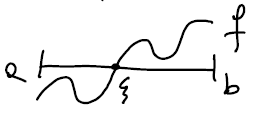
\includegraphics[width=0.3\textwidth]{pagina8_1.png}\par
$\uparrow$ \\
non è ne monotona ne convessa o concava ma $\xi$ è unico\\
\end{center}
Fatti questi brevi richiami teorici su $\exists!$ delle soluzioni di equazioni scritte nella forma 
\[f(x)=0, \quad x \in [a,b]\]
introduciamo uno dei metodi più semplici per la soluzione numerica, il \textbf{metodo} \textbf{di} \textbf{bisezione}.

\subsection{Metodo di bisezione}
Il metodo di bisezione consiste nell'applicazione iterativa del teorema degli zeri di funzioni continue, quindi si assume che 
\[f \in C[a,b], \quad f(a)f(b)<0\]
Illustriamo graficamente la costruzione delle iterazioni
\begin{center}
            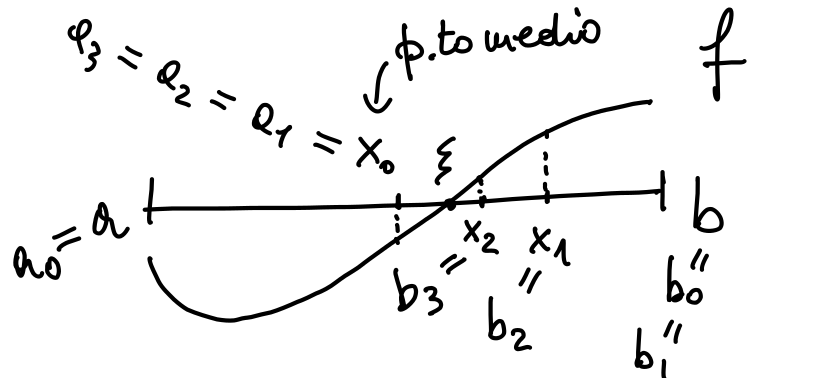
\includegraphics[width=0.5\textwidth]{im_pag10.png}\par
\end{center}
L'idea è la seguente: si parte da $[a_0,b_0]=[a,b]$, si calcola il punto medio $x_0=\frac{(a_0+b_0)}{2}$; ora se $f(x_0)=0$ siamo su uno zero; altrimenti siccome $f(a_0)$ e $f(b_0)$ hanno segno definito, $f(x_0)$ sarà discorde con uno solo dei due e quindi sicuramente ci sarà uno zero in $(a_0,x_0)$ se $f(a_0)f(x_0)<0$ altrimenti ci sarà uno zero in $(x_0, b_0)$ visto che $f(x_0)f(b_0)<0$ (sempre per il teorema degli zeri). Nel primo caso si definisce $a_1=a_0$, $b_1=x_0$, mentre nel secondo $a_1=x_0$, $b_1=b_0$, con la garanzia che $\exists \ \xi \in (a_1,b_1)$ tale che $f(\xi)=0$ visto che $f(a_1)f(b_1)<0$.

\subsubsection{Convergenza}
Il procedimento viene iterato applicando ripetutamente il teorema degli zeri per passare da $[a_n,b_n]$ ad $[a_{n+1},b_{n+1}]$ in cui uno degli estremi è diventato il punto medio $x_n=\frac{(a_n+b_n)}{2}$ di $[a_n,b_n]$.\\
Si tratta in generale di un processo infinito (a meno che per qualche $n$ non risulti $f(x_n)=0$) che permette di costruire 3 successioni $\{ a_n \} , \{ b_n \} , \{ x_n \} $ tali che:
\begin{itemize}
    \item $\exists\ \xi : f(\xi)=0, \ \xi \in (a_n,b_n)$
    \item $\abs{\,\xi - a_n\,}, \ \abs{\,\xi - b_n\,} \le b_n-a_n=\frac{b-a}{2^n}$
    \item $\abs{\,\xi - x_n\,} < \frac{b_n - a_n}{2} = \frac{b-a}{2^{n+1}}$
\end{itemize}
$n=0,1,2,\dots$ \\
Il nome ``bisezione" viene dal fatto che l'intervallo viene diviso iterativamente a metà, ``buttando via" ad ogni iterazione mezzo intervallo per restare nella metà dove $f$ cambia segno e dove quindi c'è sicuramente uno zero (``lo" zero nel caso questo sia unico in $(a,b)$, ma in generale il metodo funziona anche con vari zeri, calcolandone uno). \\
Si vede subito che il metodo è convergente, cioè che tutte e 3 le successioni convergono ad uno zero $\xi \in (a,b)$.\\
Infatti
\[0 \le \abs{\,\xi - a_n\,}, \ \abs{\,\xi - b_n\,} < \frac{b-a}{2^n}\underset{n\to \infty}{\longrightarrow}  0\]
e per il teorema dei 2 carabinieri
\[\abs{\,\xi - a_n\,}, \ \abs{\,\xi - b_n\,} \longrightarrow 0, \ n \rightarrow \infty\]
analogamente
\[\abs{\,\xi - x_n\,} \longrightarrow 0, \ n \rightarrow \infty\]
visto che 
\[0 \le \abs{\,\xi - x_n\,} < \frac{b-a}{2^{n+1}}\]
Quest'ultima diseguaglianza è immediatamente comprensibile da questo disegno
\begin{center}
    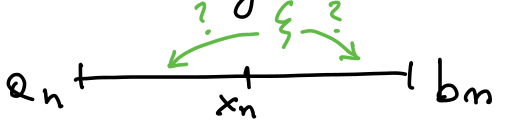
\includegraphics[width=0.5\textwidth]{6.png}\par
\end{center}
Cioè sappiamo che $\xi$ zero di $f$ sta in $(a_n, b_n)$, non sappiamo dove, ma sicuramente la sua distanza dal punto medio $x_n$ è minore di metà della lunghezza dell'intervallo $[a_n, b_n]$ cioè è $< \frac{(b_n - a_n)}{2}$, in altri termini, $\xi$ sta nell'intorno aperto di centro $x_n$ e raggio $\frac{(b_n - a_n)}{2}$. \\
Nel metodo di bisezione si sceglie $x_n$ come successione di approssimazioni, visto che la \uline{stima} dell'errore è migliore di un fattore $\frac{1}{2}$ rispetto a quella di $a_n$ e $b_n$.

\subsubsection{Stima a priori}
Volendo garantire una tolleranza di $\varepsilon > 0 $ nel calcolo approssimato del vero $\xi$, basta quindi risolvere la disuguaglianza di 
\[ e_n = \abs{\,\xi - x_n\,} < \frac{b-a}{2^{n+1}} \le \varepsilon \]
in modo che $\xi \in (x_n -  \varepsilon, x_n + \varepsilon)$, ovvero \[ 2^{n+1} \geq  \frac{b-a}{\varepsilon} \]
cioè
\[\begin{split}
   n + 1 & \ge \log_2{\frac{b-a}{\varepsilon}} \\
    & = log_2\left(b-a\right) + log_2\left(\frac{1}{\varepsilon}\right)
\end{split}\]
Questa disuguaglianza permette ``a priori", cioè prima di iniziare il processo di calcolo, di decidere a quale iterazione fermarsi in modo da garantire la tolleranza di $\varepsilon > 0$, basta prendere 
\[ n(\varepsilon) = [\log_2\left(\frac{1}{\varepsilon}\right) + log_2{(b-a)}] \quad \leftarrow \text{parte intera}\]
In effetti una stima del tipo $e_n \leq stima(n)$ dove la stima non dipende dalle quantità calcolate si chiama usualmente ``STIMA A PRIORI".\\
Il problema con le stime a priori è che sono spesso SOVRASTIME, cioè non sono vicine all'errore effettivo ma ne danno solo un confine superiore garantito in modo teorico, che però può portare ad un aumento del numero di iterazioni e quindi del costo computazionale, rispetto a quello che sarebbe sufficiente ad ottenere la tolleranza richiesta.

\subsubsection{Stima a posteriori - residuo pesato}
Per ottenere una stima dell'errore più aderente, cominciamo col fare la seguente osservazione: visto che $x_n \to \xi,\,n\to \infty$ e che $f$ è continua, si avrà che \[f(x_n) \to f(\xi)=0,\quad n \to \infty\]
Quella che stiamo usando qui in realtà è una caratterizzazione della continuità di una funzione in analisi matematica: $f$ è continua in $l$ \uline{se e solo se}
\[\forall \{x_n\}:\lim_{n\to \infty}x_n=l \text{ si ha} \lim_{n\to \infty}f(x_n)=f(l)\]
che si esprime anche dicendo ``$f$ è continua se e solo se il limite si può trasportare 'dentro' la funzione".\\
Nel nostro caso $f(\xi)=0$ quindi $f(x_n) \to 0,\,n \to \infty$ e anche $\abs{\,f(x_n)\,}\to 0,\,n \to \infty$.\\
La quantità $\abs{\,f(x_n)\,}$ si chiama ``RESIDUO" perchè dice quanto ``resta" ad $f$ per annullarsi.\\
Viene allora spontanea questa domanda: siccome $f(x_n) \to 0,\,n \to \infty$, possiamo arrestare il processo di calcolo quando il residuo $\abs{\,f(x_n)\,}$ è piccolo? In altre parole
\[\abs{\,f(x_n)\,}\le \varepsilon \overset{?}{\Longrightarrow} e_n \le \varepsilon\]
La risposta è \uline{NO}, in realtà\\
\[\abs{\,f(x_n)\,}\le \varepsilon \nRightarrow e_n\le \varepsilon\]
perchè come vedremo subito la grandezza del residuo non è in se' un buon indicatore dell'errore, ma va opportunamente ``pesata": per capirlo consideriamo i seguenti grafici\\
\begin{center}
    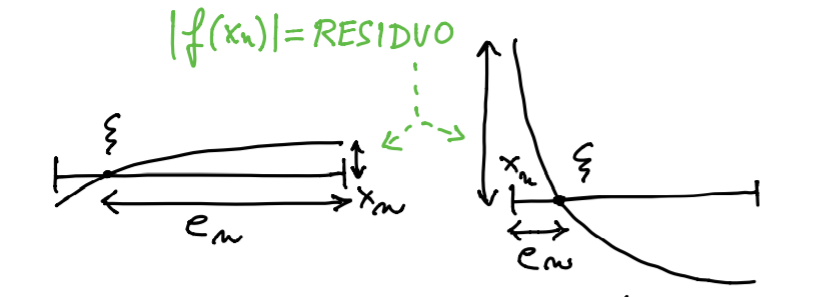
\includegraphics[width=0.6\textwidth]{grafo4.png}
\end{center}
Nel primo caso il residuo è piccolo ma l'errore è grande (cioè il residuo è una \uline{SOTTOSTIMA} dell'errore).\\
Nel secondo caso il residuo è grande ma l'errore è piccolo (cioè il residuo è una \uline{SOVRASTIMA} dell'errore).\\
È importante osservare che una \uline{sottostima} dell'errore in pratica è la cosa più \uline{pericolosa}, perchè induce a fermare le iterazioni quando $x_{n}$ non è ancora nell'intorno del limite individuato dalla tolleranza: si pensa di aver approssimato la quantità limite a meno della tolleranza e invece \uline{l'errore è più grande della tolleranza}.\\
Questo può chiaramente portare a conseguenze gravi in applicazioni in cui il rispetto della tolleranza è decisivo.
D'altra parte, una \uline{sovrastima} pur essendo meno grave, ha come conseguenza un aumento del numero di iterazioni rispetto a quello che sarebbe sufficiente e quindi un \uline{incremento} del \uline{costo computazionale}.\\
Nei due grafici disegnati sopra si nota che il residuo è una sottostima dell'errore quando la funzione è ``piatta", cioè la variazione è lenta in un intorno dello zero, mentre è una sovrastima quando la funzione è ``ripida", cioè ha una variazione veloce in un intorno dello zero.
Si capisce allora che il residuo va in qualche modo ``pesato" per tener conto della velocità di variazione: se $f$ è derivabile, bisogna quindi tenere conto della grandezza della derivata, che per definizione misura la velocità di variazione di una funzione per fare questo in modo rigoroso possiamo ricorrere a un teorema chiave del calcolo differenziale, il teorema del VALOR MEDIO (detto anche teorema di Lagrange).

\subsubsection{TEOREMA (del valor medio)}
\begin{center}
    \fbox{\begin{minipage}[t]{15cm}%
        Sia $f \in C[\alpha,\beta]$ derivabile in $(\alpha,\beta)$
        allora 
        \begin{center}
        $\exists\, z\in (\alpha,\beta)$ tale che $\frac{f(\beta) - f(\alpha)}{\beta - \alpha} = f'(z)$
        \end{center}
    \end{minipage}}
\end{center}
Interpretazione geometrica
\begin{center}
   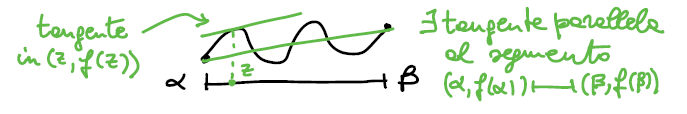
\includegraphics{pag25} 
\end{center}
Tornando all'analisi del residuo nel metodo di bisezione, mettiamoci nelle seguenti ipotesi: $f\in C^1[a,b]$ (cioè $f$ è derivabile con derivata prima continua in $[a,b]$), $\{x_n\}\subset[c,d]\subseteq[a,b]$ (almeno per $n\ge n_0$ cioè per $n$ abbastanza grande) con \[x_n \to \xi,\,n \to \infty,\,f(\xi)=0 \text{ e } f'(x)\ne 0\quad \forall x\in [c,d]\] allora vale la rappresentazione:
\[e_n = \abs{\,x_n-\xi\,} = \frac{\abs{\,f(x_n)\,}}{\abs{\,f'(z_n)\,}},\quad n\ge n_0\] con $z_n\in int(x_n,\xi)$, l'intervallo aperto che ha per estremi $x_n$ e $\xi$ (potrebbe essere $(x_n,\xi)$ oppure $(\xi,x_n)$ a seconda che $x_n<\xi$ oppure $x_n>\xi$).
\newline \newline
Prima di dimostrare la stima, osserviamo che
\begin{enumerate}
    \item la rappresentazione dell'errore mostra chiaramente che l'\uline{ERRORE} è un \uline{RESIDUO PESATO} della derivata;
    \item l'ipotesi che $f'(x)\ne0$ in $[c,d]\subseteq [a,b]$ è equivalente all'ipotesi che lo zero sia SEMPLICE, ovvero che $f'(\xi)\ne 0$ (la terminologia viene dalle equazioni algebriche, cioè quelle in cui $f$ è un polinomio, lì zero semplice significa che $(x-\xi)^{\alpha}$ compare con $\alpha =1$ nella fattorizzazione di Ruffini). Infatti, se $x_n\in [c,d]\quad \forall n>n_0$ allora $\xi=\lim x_n\in [c,d]$ perchè $[c,d]$ è chiuso e quindi contiene i limiti delle successioni lì contenute, quindi $f'(\xi)\ne 0$.
    Viceversa, se $f'(\xi)\ne 0$ siccome $f'$ è continua, per il teorema della \uline{permanenza del segno}
    \[\exists\, \delta>0 : f'(x)\ne 0\quad \forall x \in [\xi - \delta, \xi + \delta] = [c,d]\]
    e siccome $x_n \to \xi,\,n \to \infty\quad \exists \,n_0$ tale che $|x_n-\xi|\le \delta \quad \forall n \ge n_0$\\
    Si noti che $f'(z_n)\ne 0,\, n\ge n_0$ perchè $z_n \in int(x_n,\xi)\subset[c,d]$.\\
    È importante osservare che la rappresentazione dell'errore come residuo pesato non vale solo per il metodo di bisezione, ma per ogni metodo convergente a uno zero semplice se $f\in C^1$ (applicheremo infatti questo risultato più avanti al metodo di Newton)
    \item dalla rappresentazione siamo in grado di ricavare delle STIME A POSTERIORI dell'errore (a posteriori perchè si utilizza il residuo che è calcolabile solo a posteriori dopo aver prodotto $x_n$ nel processo di calcolo)
\end{enumerate}
\begin{proof}[\unskip\nopunct]
\uline{DIMOSTRAZIONE} della rappresentazione utilizzando il teorema del valor medio e supponendo che $x_n>\xi$ (l'altro caso è del tutto analogo), con $\alpha=\xi, \beta=x_n$
\[ f(x_n)-f(\xi) = f'(z_n)(x_n-\xi), \text{ } z_n \in (\xi,x_n)\]
con $f(\xi)=0$, cioè
\[ \abs{\,f(x_n)\,} = \abs{\,f'(z_n)\,}\abs{\,x_n-\xi\,} \]
che si può riscrivere come
\[ e_n = \abs{\,x_n-\xi\,} = \frac{\abs{\,f(x_n)\,}}{\abs{\,f'(z_n)\,}} \]
\end{proof}

Ora, siccome il teorema del valor medio non dice chi sia $z_n$ ma solo che esiste almeno un $z_n$ in $int(x_n,\xi)$, cerchiamo di ricavare delle stime ``pratiche" dell'errore utilizzando il residuo opportunamente pesato.

\begin{enumerate}[label=\roman*)]
\item Se è noto che $\abs{\,f'(x)\,} \ge k >0$ $\forall x \in [a,b]$ (ma basta $\forall x \in [c,d]$), allora
\[e_n = \frac{\abs{\,f(x_n)\,}}{\abs{\,f'(z_n)\,}} \underset{\underset{\underset{rigorosa}{stima}}{\uparrow}}{\le} \frac{|f(x_n)|}{k} \]

\item Se $f'$ è nota o calcolabile, siccome $z_n \to \xi, n \to \infty$ per il teorema dei 2 carabinieri visto che $z_n$ sta fra $\xi$ e $x_n$, per la continuità di $f'$ si ha che
\[ \abs{\,f'(x_n)\,}, \, \abs{\,f'(z_n)\,} \underset{n \to \infty}{\longrightarrow} \abs{\,f'(\xi)\,} \ne 0 \]
Quindi, almeno per $n$ abbastanza grande, $\abs{\,f'(x_n)\,}$ e $\abs{\,f'(z_n)\,}$  saranno entrambi dell'ordine di grandezza di $\abs{\,f'(\xi)\,}$ (notiamo che nel residuo pesato quello che interessa è essenzialmente \uline{l'ordine di grandezza del} \uline{peso} $\abs{\,f'(z_n)\,}$: per fissare le idee, sto dividendo per $100$ o per $\frac{1}{100}$? Cioè, sto ``aggiustando" una sovrastima o una sottostima?).\\
Abbiamo quindi una ``STIMA EMPIRICA":
\[ e_n = \abs{\,x_n-\xi\,} \approx \frac{\abs{\,f(x_n)\,}}{\abs{\,f'(x_n)\,}} \] 
valida almeno per $n \ge \bar{n}$, dove $\bar{n}$ corrisponde ad un controllo empirico che l'ordine di grandezza di $\abs{\,f'(x_n)\,}$ si stia ``stabilizzando", cioè valga:
\[ \abs*{\,\frac{\abs{\,f'(x_n)\,}}{\abs{\,f'(x_{n-1})\,}}-1\,} \le \delta \]


Ad esempio con $\delta = 10^{-1}$ o $10^{-2}$ $\left(\frac{\abs{\,f'(x_n)\,}}{\abs{\,f'(x_{n-1})\,}} \to 1,\ n \to \infty \right)$, quindi ha senso controllare quando il rapporto si sta stabilizzando intorno a $1$, tenendo presente che questo è un criterio sensato ma non completamente rigoroso, diciamo una ``linea guida" per l'utilizzo del peso.

\item Se $f'$ non è vuota esplicitamente, va in qualche modo approssimata.\\Osserviamo infatti che non sempre abbiamo a disposizione una formula analitica per $f$ (come ad es. per l'equazione algebrica $x^2-2=0$ corrispondente al calcolo di $\sqrt{2}$ o per l'equazione non algebrica $x-e^{-x}=0$)\\
Infatti $f$ potrebbe essere nota in forma di ``scatola nera"\\
\begin{center}
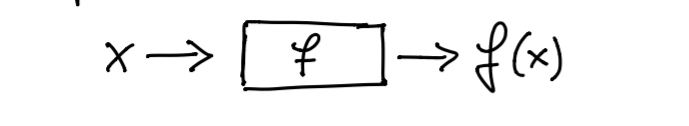
\includegraphics[width=0.5\textwidth]{scatolanera.PNG}    
\end{center}
cioè potremmo avere a disposizione solo i valori da misure o da altri algoritmi. Se però sappiamo almeno che $f$ è derivabile, possiamo approssimare $f'$ con un rapporto incrementale costruito con le quantità calcolate 
\[f'(z_n)\approx \vartheta_n=\frac{f(x_n)-f(x_{n-1})}{x_n-x_{n-1}}\overset{\overset{\overset{VALOR}{MEDIO}}{\downarrow}}{=} f'(\mu_n)\]
dove $int(x_n,x_{n-1})\ni \mu_n \rightarrow \xi, n\rightarrow\infty$ e quindi 
\[\abs{\,\vartheta_n\,}\approx \abs{\,f'(\xi)\,} \approx\abs{\,f'(z_n)\,}\] almeno per $n$ abbastanza grande: di nuovo, possiamo usare un criterio empirico per ``accettare" il valore di $\abs{\,\vartheta_n\,}$ come peso, tipo $\abs*{\,\frac{\abs{\,\vartheta_n\,}}{\abs{\,\vartheta_{n-1}\,}}-1\,}\le \delta$ 

Detto $k_n$ il peso calcolato con uno degli approcci $(i)-(iii)$, siamo allora in grado di scrivere un ``\uline{test di arresto}" per il metodo di bisezione che \uline{combina} stima \uline{a priori} e stima \uline{a posteriori}
\[min\left\{\frac{b-a}{2^{n+1}},\frac{\abs{\,f(x_n)}\,}{k_n}\right\}\le \varepsilon\]
\end{enumerate}
Possiamo a questo punto fare alcune considerazioni di carattere computazionale.

\begin{enumerate}[label=\Alph*)]
\item il metodo di bisezione funziona con \uline{richieste} analitiche e computazionali \uline{minime}.
La versione base con la stima a priori chiede solo che siano soddisfatte le ipotesi del teorema degli zeri (continuità e cambio segno agli estremi) e unicamente la possibilità di calcolare correttamente il segno di $f(x_n)$ (per cui è sufficiente un errore relativo $<100\%$ su $f(x_n)!$). Infatti in generale se 
\[\tilde{\alpha} \approx \alpha \ne 0 \quad \text{e} \quad \frac{\abs{\,\alpha-\tilde{\alpha}\,}}{\abs{\,\alpha\,}}<1 \quad \Longrightarrow \quad sign(\tilde{\alpha})=sign(\alpha)\]

\item mentre la stima a priori è decrescente, l'errore effettivo in generale non lo è, come si vede da questo disegno
\begin{center}
    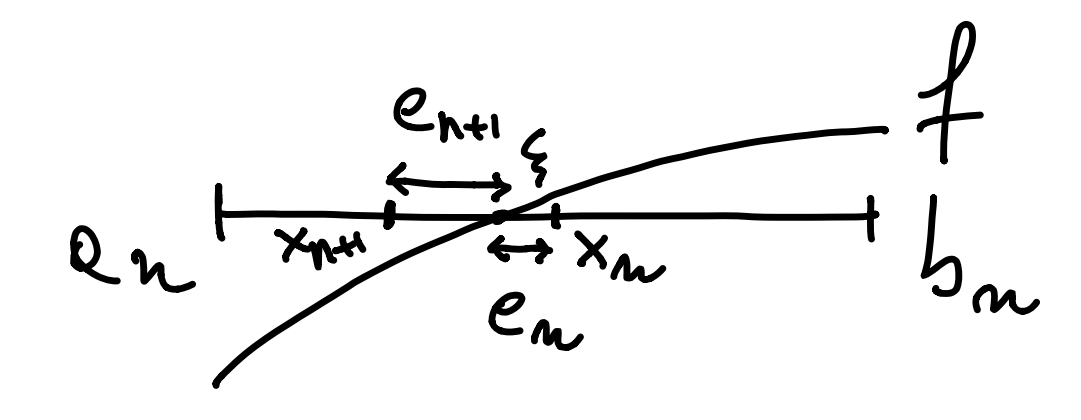
\includegraphics[width=0.5\textwidth]{grafo3.png}\par
\end{center}
 dove $e_{n+1}>e_n$ ( anche se comunque $e_n \rightarrow 0, n \rightarrow \infty$); qui si vede anche che $e_n\ll\frac{(b_n-a_n)}{2}$ e la stima del residuo pesato è tendenzialmente più accurata. A differenza della stima a priori che si dimezza, $e_{n+1}\approx\frac{e_n}{2}$ solo ``in media" su un po' di iterazioni.
\end{enumerate}

Concludiamo la lezione con un esempio, il calcolo approssimato di $\sqrt{2}$ risolvendo l'equazione algebrica $x^2 -2 = 0$ con il metodo di bisezione.\newline

\subsubsection{Calcolo di $\sqrt{2}$ alla precisione di macchina}
Consideriamo l'equazione algebrica
\[f(x)=x^2-2=0\] Calcolarne la soluzione positiva significa calcolare $\sqrt{2}$. Le ipotesi del teorema degli zeri sono soddisfatte in $[a,b]=[1,2]$.\\
Infatti $f\in C[a,b]$ (anzi $f\in C^{\infty}(\mathbb{R})$ cioè è derivabile infinite volte in $\mathbb{R}$ con derivate tutte continue, perché $f$ è un polinomio) \[f(a)=f(1)=1-2=-1<0\] \[f(b)=f(2)=2^2-2=2>0\]
Inoltre $f'(x)=2x \geq 2\quad\forall x \in [1,2]$ quindi $\sqrt{2}\in (1,2)$ ed è l'unico zero in tale intervallo (in effetti sappiamo che è l'unico zero in $\mathbb{R}^+$)
possiamo applicare il metodo di bisezione che comincia in questo modo: 
\[\begin{split}
    x_0 & = \frac{1+2}{2} = 1.5, \\
    x_1 & = \frac{1+1.5}{2} = 1.25, \\
    x_2 & = \frac{1.25+1.5}{2} = \frac{2.75}{2} = 1.375, \\
    x_3 & = \frac{1.375+1.5}{2} = 1.4375, \\
    \dotso
\end{split}\]
(ricordiamo che $\sqrt{2}=1.4142\dots$).\\
Nel grafico sottostante (in scala log) riportiamo l'errore effettivo, la stima a priori \[\frac{(b_n-a_n)}{2}=\frac{1}{2^{n+1}}\] 
e la stima a posteriori
\[\frac{\abs{\,f(x_n)\,}}{k}=\frac{\abs{\,x_n^2-2\,}}{2}\]
(visto che $f'(x)\ge k=2 \quad \forall x\in [1,2]$) tutte relativizzate a $\abs{\,\xi\,}=\sqrt{2}$ (in questo caso comunque $\abs{\,\xi\,}$ è dell'ordine dell'unità e quindi errore assoluto e relativo vicini)
\begin{center}
    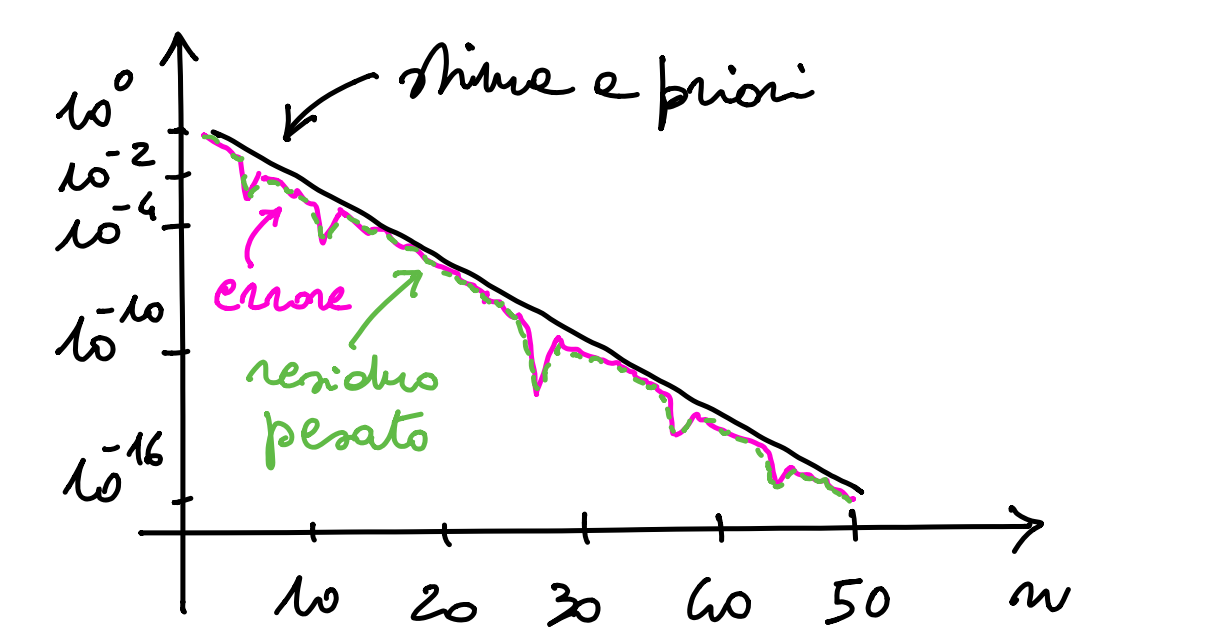
\includegraphics[width=0.5\textwidth]{grafo2.png}\par
\end{center}
(come sempre per comodità i valori discreti sono interpolati con linee continue o tratteggiate).\\
Si vede che l'errore segue solo ``in media" l'andamento della stima a priori, che la sovrastima a volte di vari ordini di grandezza (picchi dell'errore verso il basso, ad esempio tra $n=20$ e $n=30$ l'errore va circa a $10^{-11}$ mentre la stima a priori ha bisogno di una decina di iterazioni in più).\\
D'altra parte la stima del residuo pesato è praticamente sovrapposta all'errore effettivo.\\
Si noti infine che per raggiungere un errore dell'ordine della precisione di macchina $\varepsilon_M=2^{-53}$ servono circa $50$ iterazioni, il che non è sorprendente visto che il fattore medio di riduzione dell'errore è $\frac{1}{2}$.

\end{document}
